\documentclass[a4paper,12pt,leqno]{article}
\usepackage[utf8]{inputenc}
\usepackage[ngerman]{babel}

\usepackage{amsmath}
\usepackage{amsthm}
\usepackage{amsfonts}
\usepackage{amssymb}
\usepackage[left=3cm,right=2cm,top=2cm,bottom=1.5cm]{geometry}
\usepackage{parskip}
\usepackage{graphicx}
\usepackage{caption}
\usepackage{hyperref}
\usepackage{upgreek}
\usepackage{mathtools}
\usepackage{tikz}
\hypersetup{
    colorlinks,
    citecolor=black,
    filecolor=black,
    linkcolor=red,
    urlcolor=red
}

%%Code style
\usepackage{listings}
\usepackage{xcolor}
\definecolor{codegreen}{rgb}{0,0.6,0}
\definecolor{codegray}{rgb}{0.5,0.5,0.5}
\definecolor{codepurple}{rgb}{0.58,0,0.82}
\definecolor{backcolour}{rgb}{0.9,0.9,0.9}

\lstset{escapeinside={@}{@}}
\lstdefinestyle{mystyle}{
    backgroundcolor=\color{backcolour},   
    commentstyle=\color{codegreen},
    keywordstyle=\color{magenta},
    numberstyle=\tiny\color{codegray},
    stringstyle=\color{codepurple},
    basicstyle=\ttfamily\footnotesize,
    breakatwhitespace=false,         
    breaklines=true,                 
    captionpos=b,                    
    keepspaces=true,                 
    numbers=left,                    
    numbersep=5pt,                  
    showspaces=false,                
    showstringspaces=false,
    showtabs=false,                  
    tabsize=5
}

\lstset{style=mystyle}

\newcommand{\blue}[1]{\textcolor{blue}{#1}}
\newcommand{\orange}[1]{\textcolor{orange}{#1}}
\newcommand{\violet}[1]{\textcolor{violet}{#1}}
%%End code style

\title{Computer System Sicherheit\\Notizen WS20/21}
\author{Felix Marx}

\begin{document}
\maketitle

{
%%Lokales Einfärben des Inhaltverzeichisses
\hypersetup{linkcolor=black}
\tableofcontents
}
\newpage

\section{Begriffe}
Unterscheidung \blue{Betriebssicherheit (safety)} und \blue{Angriffssicherheit (security)}.\\
safety bezeichnet den Schutz vor inneren Fehlern, deren Eintrittswahrscheinlichkeit durch probabilistische Techniken ermittelt wird.\\
security den Schutz gegen aktive Angreifer.

\subsection{Security}

Trends und Herausforderungen:\\
\textbf{Mobilität}, der Übergang zu ''smart devices''
\begin{figure}[h!]
\centering
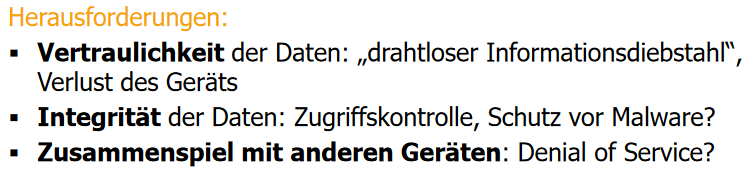
\includegraphics[scale=0.6]{Grafiken/Trend-Mobilitaet.png}
\caption{Herausforderungen bei der Mobilität}
\end{figure}

\textbf{Vernetzung}, der Übergang zu ''always on'' und Automatisierung von Systemen
\begin{figure}[h!]
\centering
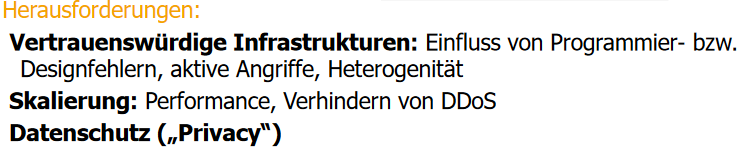
\includegraphics[scale=0.6]{Grafiken/Trend-Vernetzung.png}
\caption{Herausforderungen bei der Vernetzung}
\end{figure}

\textbf{Miniaturisierung}, Produktion kleinerer Chips mit Trend zu Einwegchips
\begin{figure}[h!]
\centering
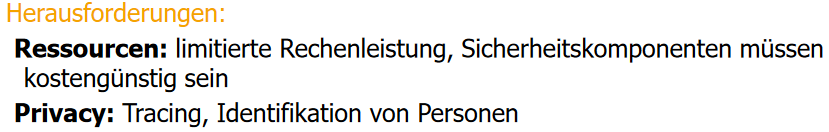
\includegraphics[scale=0.6]{Grafiken/Trend-Miniaturisierung.png}
\caption{Herausforderungen bei der Miniaturisierung}
\end{figure}\\

\blue{Social Engineering} bezeichnet das Erlangen von vertraulichen Daten durch psychologische Techniken\\
\blue{Man-in-the-middle} Angriffe, hier werden Nachrichten vor der gesicherten Kommunikation abgefangen.\\
Lösungen für \blue{Phishing} umfassen die Verifikation durch Transaktionsnummern (TANs) oder Hardwaretokens was allerding nicht die Integrität der Transaktion gewährleistet.\\
Schutzmechanismen:\\
\blue{Passive Authentication}: Sicherstellung der Authentizität durch Einsatz einer digitalen Signatur\\
\blue{Basic Access Control}: elektronische gespeicherte Daten werden erst übermittelt wenn das Lesegerät einen aufgedruckten maschinenlesbaren Code kennt.\\
\blue{Active Access Control}: Verhindert 1:1 Kopien indem ein geheimer Schlüssel in einem gesicherten Chip-Bereich gespeichert wird.\\
\blue{Extended Access Control}: Schutz von sensiblen Daten (Fingerabdruck, Iris, etc.) durch das Abgleichen von \href{https://en.wikipedia.org/wiki/Extended_Access_Control}{Zertifikaten} die nur eine kurze Zeit gültig sind.

\subsection{Safety}
Im Fehlerfall sollte ein System immer in den sicheren Zustand übergehen.\\
Zum Beispiel zeigt die Fahranweisung von Zügen nach oben, sodass es bei einem Schaden am Mechanismus in den Haltezustand nach unten fällt (Schwerkraft). Ein Watchdog (hier Schwerkraft) überwacht quasi das System auf Fehler und resettet es bei einem Fehler.

\section{Verlässliche Systeme}
Ein zuverlässiges System erfüllt seinen Zweck auch falls Fehler auftreten.
\begin{figure}
\centering
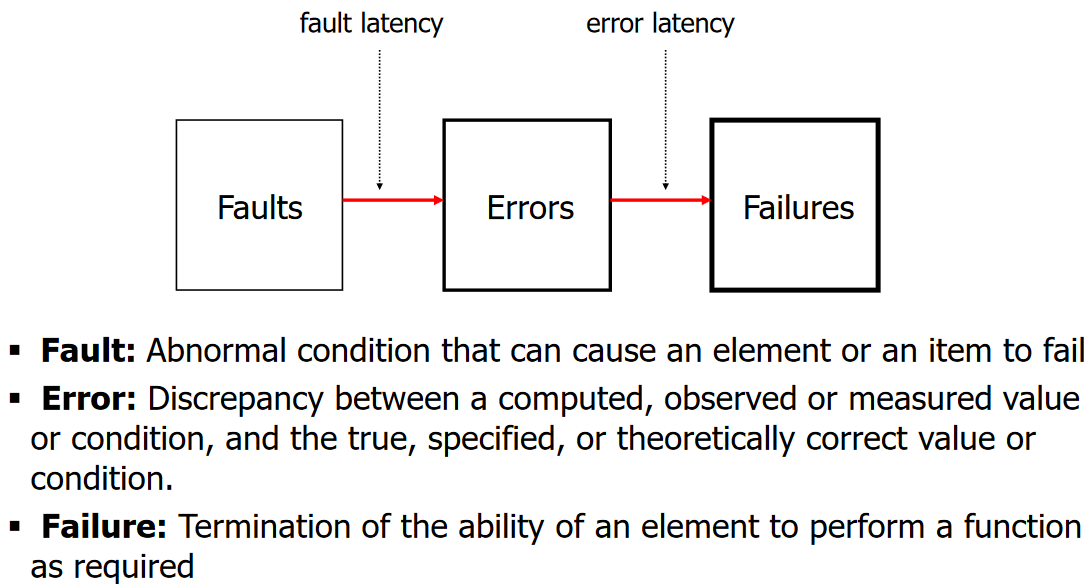
\includegraphics[scale=0.4]{Grafiken/AblaufZumVersagen.png}
\caption{Ablauf bis ein System versagt}
\label{Image:Versagensplan}
\end{figure}
Als Beispiel des \hyperref[Image:Versagensplan]{Ablaufes} lässt sich die Einwirkung von kosmischer Strahlung auf eine DRAM-Zelle (Fault) was zum Wechsel eines Wertes führt (Error), wodurch die Berechnung ein falsches Ergebnis liefert (Failure).\\
In der Zuverlässigkeit wird unterschieden nach:\\
\textbf{Availability}: Verfügbarkeit eines Systems gemessen in Prozent, d.h. 
$$\frac{\textrm{Total Up Time}}{\textrm{Total (Up + Down Time)}}=\frac{\textrm{MTTF}}{\textrm{MTTF + MTTR}}$$
\textbf{Reliability}: Zuverlässigkeit eines Systems, d.h. die Wahrscheinlichkeit dass ein System über einen gewissen Zeitraum korrekt funktioniert.\\
Wir bezeichnen mit \blue{MTTF} die Mean Time To Failure und mit \blue{MTTR} Mean Time To Recovery. Bei der Berechnung wird für die Up/Downtime nur die Zeiten im vereinbarten Betriebszeitraum gezählt!\\
Die Wahrscheinlichkeit, dass ein System bis zum Zeitpunkt $t$ fehlerhaft wird lässt sich mittels einer Verteilerfunktion $F$ und der Lebenszeit des Systems T berechnen:
$$F(t)=P(T\leq t)\textrm{, } R(t)=P(T>t)=1-F(t)$$
Die Funktion $R$ hingegen ermittelt die Wahrscheinlichkeit, dass ein System bis zum Zeitpunkt $t$ korrekt funktioniert.
Geht man davon aus, dass zukünftige Ausfälle unabhängig davon passieren, wann der letzte Ausfall war, lässt sich die Wahrscheinlichkeit mit einer Fehlerrate $\lambda$ so ausdrücken:\\
\begin{align*}
f(x) = &
\begin{cases} 
	\lambda e^{-\lambda x} & x\geq 0\\
	 0 & x < 0
\end{cases} \\
F(t) = & \int_{-\infty}^t f(x)dx = &
\begin{cases}
1 -e^{-\lambda t} & t \geq 0\\
0 & t < 0
\end{cases}\\
R(t) = & 1 -F(t) = & 
\begin{cases}
e^{-\lambda t} & t \geq 0\\
1 & t< 0
\end{cases}
\end{align*}
\begin{figure}[h!]
\centering
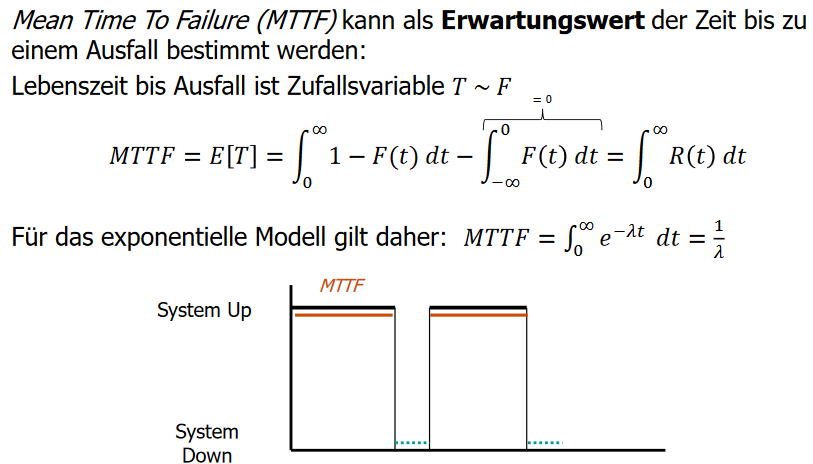
\includegraphics[scale=0.6]{Grafiken/MTTF-Model.png}
\caption{Berechnung MTTF mit dem exponentiellen Model}
\end{figure}\\
Bei in Reihe geschalteten Komponenten wird die Wahrscheinlichkeit dass das gesamte System korrekt funktioniert R durch $R_{ges}(t)=\prod^n_{i=1}R_i(t)$ im exponentiellen Modell wird dann für $\lambda = \lambda_{ges}=\sum_{i=1}^n\lambda_i$ verwendet.\\
Bei Parallelschaltung ist die Wahrscheinlichkeit dass das System korrekt funktioniert:
$$R_{ges}(t)=R_1(t)+R_2(t)-R_1(t)\cdot R_2(t), F_{ges}(t)=F_1(t)\cdot F_2(t)$$
Bei mehr als zwei Komponenten ist die allgemeine Formel:
$$R_{ges}(t)=1-\prod_{i=1}^n(1-R_i(t)), F_{ges}(t)=\prod_{i=1}^nF_i(t)$$

\subsection{Strategien zur Fehlervermeidung/toleranz}
\begin{itemize}
\item Fehlervermeidung (fault avoidance)
	\begin{itemize}
	\item Design des Systems stellt sicher, dass Fehler nicht auftreten
	\item Beispiel: Testen, Verifikation,...
	\end{itemize}
\item Wiederherstellung aus Fehlerzustand (fault recovery)
	\begin{itemize}
	\item Strategien, um ein System beim Auftreten eines Fehlers wieder in einen korrekten Systemzustand zu bringen
	\end{itemize}
\item Fehlertoleranz (fault tolerance)
	\begin{itemize}
	\item Wenn Fehler nicht vermieden werden können, dann soll das System Fehler tolerieren
	\item Beispiele: Redundanz, Safety, ...
	\end{itemize}
\end{itemize}
\textbf{Arten von Redundanzen:}
\begin{itemize}
\item Physikalische Redundanz (physical redundancy)
	\begin{itemize}
	\item Zusätzliche Ressourcen bzw. Komponenten
	\item Berechnungen werden auf mehreren Komponenten ausgeführt und verglichen
	\item Statische Redundanz
		\begin{itemize}
		\item $N$ Systeme laufen parallel
		\item $N-1$ Systeme laufen im  ''stand-by-mode''
		\item Bei einem Fehler wird im Betrieb umgeschaltet
		\item Dazu muss man den Fehler natürlich zuerst erkennen!
		\end{itemize}
	\item Dynamische Redundanz
		\begin{itemize}
		\item $N$ Systeme laufen parallel
		\item Ausfallsicherhere Komponente vergleicht die Resultate
		\item Mehrheitsentscheidung (zB. 2-out-of-3)
		\item Erkennt Fehler ''automatisch''
		\end{itemize}
	\end{itemize}
\item Zeitliche Redundanz (temporal redundancy)
	\begin{itemize}
	\item Berechnungen auf gleicher Hardware-Plattform wiederholen
	\end{itemize}
\item Redundanzen durch (Zusatz-)Information (information redundancy)
	\begin{itemize}
	\item Hinzufügen von zusätzlichen Daten (Checksummen, ...)
	\item Erlaubt Datenfelder bei Übertragung oder Speicherung zu erkennen
	\end{itemize}
\end{itemize}
Bei dynamischer Redundanz wird das Ergebnis parallel berechnet und dann per Mehrheitsentscheidung das korrekte ausgewählt. Problematisch falls im Vergleich ein Problem auftritt. Softwarefehler sind von der Hardware-Redundanz nicht abgedeckt.
Zusatzinformationen können die Integrität gesendeter Daten durch Checksummen sicherstellen, allerdings auch nur begrenzt.\\

Nachteile von Redundanzen sind:
\begin{itemize}
\item Schlechtere Performanz (bei temporaler Redundanz)
\item Synchronisation erforderlich
\item Hohe Kosten durch mehrfache Hardware bzw. mehrfache Implemenation (falls überhaupt möglich)
\item Benötigt Mechanismen zur Fehler-Erkennung, welche selbst wieder Fehleranfällig sein können
\end{itemize}

\section{Krypographie}
\begin{itemize}
\label{item:schutzziele}
\item Vertraulichkeit (Confidentiality)
	\begin{itemize}
	\item Schutz vor unbefugten Zugriff auf Informationen / Daten
	\end{itemize}
\item Integrität
	\begin{itemize}
	\item Schutz vor Veränderung von Informationen / Daten
	\end{itemize}
\item Verfügbarkeit (Availability)
	\begin{itemize}
	\item Daten oder Systeme sind verfügbar oder erreichbar
	\end{itemize}
\item Authentizität (Authenticity)
	\begin{itemize}
	\item Garantie dass die Daten auch aus der angegebenen Quelle stammen
	\end{itemize}
\item Nicht-Abstreitbarkeit (Non-Repudiation)
	\begin{itemize}
	\item Aktion ist nachprüfbar und kann nicht abgestritten werden
	\end{itemize}
\end{itemize}
\subsection{Begriffe}
\begin{itemize}
\item Klartext/Nachricht: eine zu verschlüsselnde Information
\item Klartextraum: Menge aller möglichen Klartexte
\item Chiffrat, Chiffretext: Verschlüsselte Nachricht
\item Chiffretextraum: Menge aller möglichen Chiffrate
\item Schlüssel: Ein Geheimnis, welches zur Ent-/Verschlüsselung benötigt wird
\item Schlüsselraum: Menge aller möglichen Schlüssel
\item Verschlüsselung: Umwandlung eines Klartext in ein Chiffrat
\item Entschlüsselung: Umwandlung eines Chiffrats in einen Klartext
\end{itemize}
\textbf{Kerckhoffs Prinzipien}
\begin{enumerate}
\item Das System muss praktisch, wenn nicht sogar mathematisch, unentschlüsselbar sein (''Unentschlüsselbarkeit'')
\item Es darf keine Geheimhaltung erfordern und darf ohne Schwierigkeiten  in die Hände des Feindes fallen (''Keine Geheimhaltung des Systems'')
\item Der Schlüssel muss ohne Hilfe geschriebener Notizen kommunizierbar und aufbewahrbar sein und er muss ausgewechselt oder modifiziert werden können nach Belieben der Kommunikationspartner (''Schlüssel ohne Aufschreiben'')
\item Es muss anwendbar sein auf die telegraphische Kommunikation
\item Es soll protabel sein und seine Funktion soll nicht die Zusammenkunft mehrerer Personen erfordern 
\item Schließlich ist es notwendig, angesichts der Umstände, unter denen es angewendet werden soll, dass das System einfach benutzbar ist und weder große gedankliche Anstrengung erfordert noch die Kenntnis einer langen Liste zu beachtender Regeln (''einfach benutzbar'')
\end{enumerate}
\subsection{Verschiebechiffre}
Die Ceasar-Chiffre ersetzt jeden Buchstaben des Klartextes durch den Buchstaben 3 Stellen weiter rechts, beim Entschlüsseln genau umgekehrt.\\
Die Verschiebechiffre ersetzt alle Buchstaben durch den Buchstaben welcher eine beliebige aber feste Anzahl an Stellen weiter rechts steht. Der Schlüssel ist die Anzahl an Verschiebungen, d.h. 0,1,2,...,25.

\subsection{Mathematische Grundlagen}
\label{def:Einwegfunktion}
Als \blue{Einwegfunktionen} bezeichnet man Funktionen deren Funktionswert $y = f(x)\in Y$ zu einem gegebenen $x$ in polynomieller Zeit berechenbar ist, aber ein Urbild $x\in f^{-1}[\{y\}]$ zu einem gegbenen $y$ nicht in Polynomialzeit bestimmbar ist. Die Existenz von Einwegfunktionen ist nicht bewiesen (P/NP).
\subsubsection{Teilbarkeitsregeln}
\begin{align}
a | a\\
a | b \wedge b |c \Rightarrow a|c\\
a|b\wedge b\neq 0 \Rightarrow |a|\leq |b|\\
a | b\wedge b|a \Rightarrow |a| = |b|
\end{align}
Sind $a,n\in\mathbb{Z}$ mit $n\neq 0$, dann gibt es eindeutig bestimmte Zahlen $q,r\in\mathbb{Z}$ sodass
\begin{align*}
a= qn+r\\
0\leq r < |n|\\
q = \lfloor \frac{a}{n} \rfloor \wedge r = a -qn
\end{align*}
\subsubsection{Größter gemeinsamer Teiler}
\label{sec:euklid}
Wir definieren $\mathbb{Z}_p^\times:=\{x\in\mathbb{Z}_p : ggT(x,p)=1\}$ als die Menge der multiplikativ Inversen in $\mathbb{Z}_p$. Ist $p$ prim, dann ist $(\mathbb{Z}_p^\times,\cdot_p,1)$ eine zyklische Gruppe.
\begin{align}
\textrm{ggT}(a,0)=|a|\\
\textrm{ggT}(a,1)=1\\
\textrm{ggT}(a,b)=\textrm{ggT}(b,a)\\
\textrm{ggT}(a,b)=\textrm{ggT}(|a|,|b|)\\
\textrm{ggT}(a,b)=\textrm{ggT}(b,a-b)\\
\textrm{Für } b\neq 0 \textrm{ gilt } \textrm{ggT}(a,b)=\textrm{ggT}(b,a \textrm{ mod } b)
\end{align}

Lineare diophantische Gleichung: $ax+by=c$\\
Eine diophantische Gleichung kann wie folgt gelöst werden.\\
Löse $ax'+by'=$ggT(a,b) und definiere $x=\frac{c}{\textrm{ggT(a,b)}}\cdot x'$, $y=\frac{c}{\textrm{ggT(a,b)}}\cdot y'$

\textbf{Beispiel erweiteter Euklid:}
$1337\cdot x+42\cdot y=\blue{7}$\\
\begin{tabular}{|l|l|l|l|l|}
a & b & $\lfloor \frac{a}{b} \rfloor$ & x & y\\
\hline
1337 & 42 & 31 & -1 & $1-31*(-1)=32$\\
\hline
42 & 35 & 1 & 1 & $0-1*1=-1$\\
\hline
35 & 7 & 5 & 0 & 1\\
\hline
\blue{7} & 0 & & 1 & 0
\end{tabular}\\
\subsubsection{Primzahlen}
Fundamentalsatz der Arithmetik:\\
Jede natürliche Zahl $n>1$ besitzt eine Zerlegung in ein Produkt aus Primzahlen, welche bis auf die Reihenfolge eindeutig ist.\\
Es gibt unendlich viele Primzahlen.\\

Die Eulersche-Phi-Funktion $$\varphi (b)=|\{a\in\mathbb{N} : a < b, \textrm{ggT}(a,b)=1\}|$$ beschreibt dei Anzahl der zu b teilerfremden Zahlen.\\
Für eine Primzahl p gilt $\varphi (p)=p-1$ und $\varphi (p^n)=p^n-p^{n-1}$.\\
Für teilerfremde Zahlen $a,b\in \mathbb{N}$ gilt $\varphi (ab)=\varphi (a)\cdot \varphi (b)$.\\
Sind $m,n\in \mathbb{N}$ teilerfremd, dann gilt $m^{\varphi (n)}\textrm{mod }n= 1$.\\
\textbf{Kleiner Satz von Fermat:}\\
Für eine Primzahl p und ein teilerfremde Zahl $m\in \mathbb{N}$ gilt $m^{p-1} \textrm{mod }p = 1$.
\subsection{Symmetrische Kryptosysteme}
In symmetrischen Kryptosystemen ist der Schlüssel zum Ver- und Entschlüsseln der selbe.\\
Formal bezeichnet ein symmetrisches Kryptosystem ein 5-Tupel $(\mathcal{M},\mathcal{K}, \mathcal{C},e,d)$ mit $\mathcal{M}$ als Menge an Klartexten, $\mathcal{K}$ als Menge von Schlüsseln, $\mathcal{C}$ als Menge an Chiffretexten.
$e: \mathcal{M}\times\mathcal{K}\rightarrow\mathcal{C}$ ist die Verschlüsselungsfunktion und $d: \mathcal{C}\times\mathcal{K}\rightarrow\mathcal{M}$ als Entschlüsselungsfunktion.\\
Weiter werden folgende Funktionen eingeführt:
\begin{align*}
num: & \{ A,B,C,...,Z\}\rightarrow\{ 0,1,2,...,25\} \textrm{ Zuordnung der Zahlenwerte}\\
char: & \{ 0,1,2,...,25\}\rightarrow\{ A,B,C,...,Z\}\\
sr: & \{A,...,Z\}\times\{0,1,...,25\}\rightarrow\{A,...,Z\} \textrm{ Ist ein Rechtsshift}\\
sl: & \{A,...,Z\}\times\{0,1,...,25\}\rightarrow\{A,...,Z\} \textrm{ Linksshift}
\end{align*}
Damit ergibt sich die für Verschiebechiffren die folgenden Interpretationen:
\begin{align*}
e(w_0w_1...w_n,k) &= sr(w_0,k)sr(w_1,k)...sr(w_n,k)\\
d(w_0w_1...w_n,k) &= sl(w_0,k)sl(w_1,k)...sl(w_n,k)
\end{align*}
Monoalphabetische Chiffretexte können durch Häufigkeitsanalysen gebrochen werden.
Um das zu verhinden existiert das \blue{One Time Pad} hierbei hat der Schlüssel die selbe Länge wie der Klartext, d.h. jeder Buchstabe im Klartext wird mit einem eigenen Schlüsselbuchstaben verschlüsselt. Das Kryptosystem sieht dann so aus: $(\mathcal{M}^n,\mathcal{K}^n, \mathcal{C}^n,e,d)$
Die Bitweise veroderung ist ein One Time Pad $(\mathbb{Z}_2^n,\mathbb{Z}_2^n,\mathbb{Z}_2^n,e,d)$ mit 
\begin{align*}
e:\mathbb{Z}_2^n\times\mathbb{Z}_2^n\rightarrow\mathbb{Z}_2^n,e(x,k)=x\oplus k\\
d:\mathbb{Z}_2^n\times\mathbb{Z}_2^n\rightarrow\mathbb{Z}_2^n,d(y,k)=y\oplus k
\end{align*}
Ein Kryptosystem heißt \blue{perfekt sicher} wenn für einen gegebenen Chiffretext jeder Klartext gleich wahrscheinlich ist, d.h. das One Time Pad ist bei gleichverteiltem zufälligen Schlüssel perfekt sicher.
Ein Kryptosystem heißt \blue{semantisch sicher}, wenn es für einen Angreifer der die Länge der Nachricht und das Chiffrat kennt nicht wesentlich einfacher ist auf den Klartext zu schließen als für einen Angreifer der nur die Länge des Klartextes kennt.\\
Als \blue{Blockchiffren} werden Kryptosysteme bezeichnet deren Klartexte $M^n$ und Chiffretexte $C^n$ alle eine Blocklänge n und deren Schlüssel $K^m$ die Schlüssellänge m haben.
Blockchiffre Verfahren sind unter anderem:
\begin{itemize}
\item Advanced Enrcyption Standard (AES) oder Rijndael
	\begin{itemize}
	\item Blocklänge: $n= 128$
	\item Schlüssellänge: $m\in \{128,192,256\}$
	\end{itemize}
\item Data Encryption Standard (DES)
	\begin{itemize}
	\item Gebrochen für $n=64$ und $m=56$
	\item 3DES mit $n=64$ und $m=168$ hat die selbe Sicherheit wie 112 Bit Schlüssel
	\end{itemize}
\item Serpent ($n=128$, $m\in\{128,192,256\}$)
\item Twofish ($n=128$, $m\in\{128,192,256\}$)
\item Blowfish ($n=64$, $32\leq m\leq 448$ - Standard: $m=128$)
\end{itemize}
\subsubsection{Vigenère mit alphabetischen Schlüssel, Länge n}
Beim Vignerère wird der Klartext entsprechend eines Codewortes verschlüsselt. Dabei wird der aktuelle Buchstabe des Klartextes um die Wertigkeit des aktuellen Buchstabens des Codewortes im Alphabet nach rechts verschoben. Ist man am Ende des Schlüsselwortes angekommen beginnt man wieder am ersten Buchstaben.\\
Verwendet man einen zufällig erstellten Schlüssel, der genauso lang ist wie der Klartext und benutzt ihn nur ein einziges Mal, so ist die Verschlüsselung perfekt sicher, kann also ohne Schlüssel nicht entschlüsselt werden (One-Time-Pad).
Zur Darstellung der Verschiebung kann ein Vigenère-Quadrat verwendet werden. Der Schlüsselraum ist $25^n$.\\
\begin{figure}[h!]
\centering
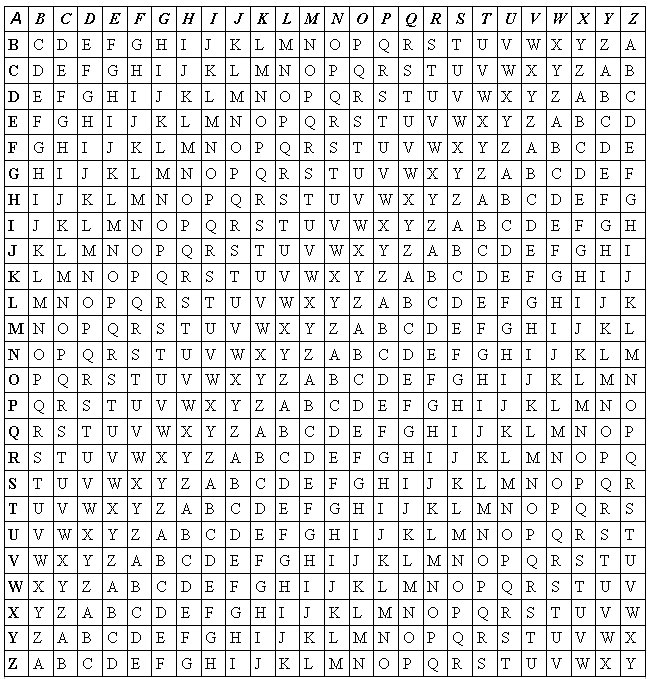
\includegraphics[scale=0.7]{Grafiken/VigenereSquare.jpg}
\caption{Vigenère Quadradt, an der X-Achse ist die Verschiebung und Y-Achse der Klarbuchstabe}
\end{figure}
\subsubsection{Electronic Codebook Modus}
Im ECB Modus werden die einzelnen Blöcke im Blockchiffre Kryptosystem jeweils mit dem selben Schlüssel verschlüsselt und die einzelnen Chiffretexte kombiniert um den gesamten Chiffretext zu bekommen. Die \hyperref[pic:ECBModus]{Entschlüsselung} läuft analog.
Da nicht alle Blöcke die genau vom Kryptosystem geforderte Länge besitzen müssen die Blöcke teilweise mit einer Auffüllfunktion $pad: M^*\rightarrow (M^n)^*$ gefüllt idealerweise sollte eine pad Funktion wieder umkehrbar sein.
Der ECB Modus ist für Klartexte welche in mehrere Blocke augeteilt werden unsicher und sollte nie verwendet werden.\\
Im ECB Modus ist die Ver- und Entschlüsselung parallelisierbar.

\begin{figure}
\centering
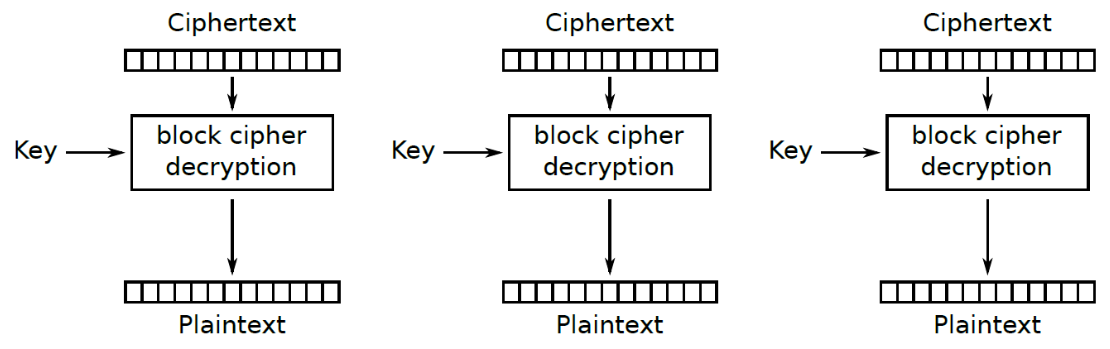
\includegraphics[scale=0.5]{Grafiken/ECBModus.png}
\caption{Entschlüsselung im ECB Modus}
\label{pic:ECBModus}
\end{figure}

\subsubsection{Cipher Block Chaining Modus}
Der CBC Modus ist eine Verbesserung des ECB Modus, da hier für die Ver- und \hyperref[fig:CBCModus]{Entschlüsselung} jeweils der vorherige Block als Rauschen mit dem Klartext verodert wird, sodass auch gleiche Muster im Klartext verschiedene Ergebnisse im Chiffretext produzieren. Dafür erweitern wir das Kryptosystem um die Menge der Zufallswerte $\mathcal{R}$ aus welcher der Initialisierungvektor gewählt wird. Hierbei ist $\mathcal{R}$ nicht geheim und kann unverschlüsselt übertragen werden.\\
Es soll $e(x,k,r_1)\neq e(x,k,r_2)$ gelten. Für die Sicherheit der Verschlüsselung ist wichtig, dass jeder Zufallswert nur einmal verwendet wird.\\
Das erweiterte Kryptosystem heißt \blue{randomisiertes symmetrisches Kryptosystem} und wird als 6-Tupel dargestellt: $(\mathcal{M},\mathcal{K},\mathcal{C},\mathcal{C},\mathcal{R},e^*,d^*)$. Der Definitionsbereich von $e^*$ und $d^*$ wird um $\mathcal{R}$ erweitert.
$$y_i = e(x_i\oplus y_{i-1},k), x_i = d(y_i,k)\oplus y_{i-1} \textrm{ für } i\geq 1$$
\begin{figure}
\centering
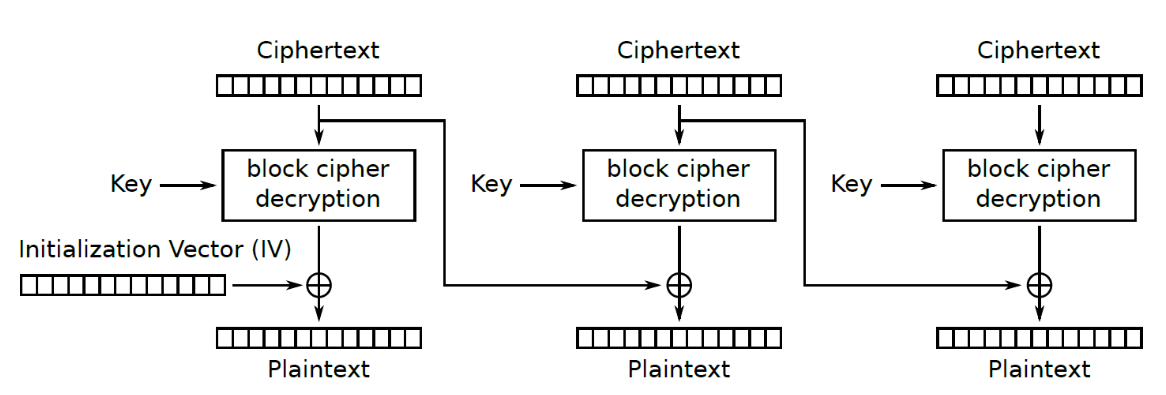
\includegraphics[scale=0.5]{Grafiken/CBCModus.png}
\caption{Entschlüsselung im CBC Modus, bei der Entschlüsselung umgedreht, sodass Parallelisierung unmöglich ist}
\label{fig:CBCModus}
\end{figure}
Die Verschlüsselung ist damit nicht mehr parallelisierbar, aber die Entschlüsselung bleibt es.\\

Damit die Verschlüsselung auch parallelisierbar ist gibt es den \blue{Counter (CTR) Modus} hier wird bei der Verschlüsselung für jeden Block der Initialiserungsvektor mit einem Zählerwert verschlüsselt und erst dann mit dem Klartext verodert. Die \hyperref[pic:CTRModus]{Entschlüsselung} läuft genau gleich ab, nur das hier der Ciffretext verodert wird.\\
\begin{figure}
\centering
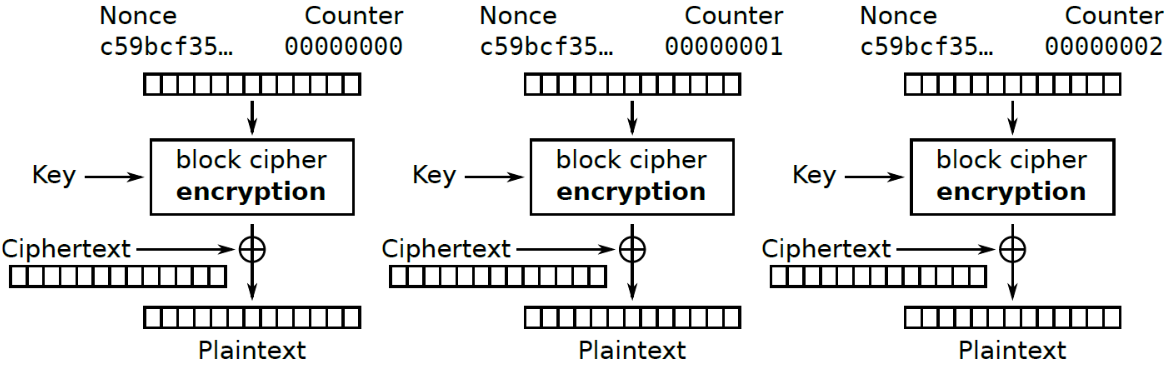
\includegraphics[scale=0.5]{Grafiken/CounterCTRModus.png}
\caption{Entschlüsselung im CTR Modus, Nonce ist der Initialiserungsvektor}
\label{pic:CTRModus}
\end{figure}
Die Wahl des Initialisierungsvektor muss unvorhersagbar sein, das heißt nicht das die Initialisierungsvektoren selber geheim bleiben müssen (die Sicherheit des Chiffretextes garantiert der Schlüssel) sondern dass die Wahl zukünftiger Initialisierungsvektoren nicht vorhersagbar sein dar (sie also von geheimen Informationen abhängen) und ein Angreifer die Wahl nicht beeinflussen kann\footnote{\url{https://tinyurl.com/y5x3bd5j} BSI Seite 76}.\\
Möglichkeiten zur Wahl des Initialisierungsvektor sind:
\begin{itemize}
\item Zufällige Initialisierungvektoren, d.h. eine zufällige Bitfolge der Länge n, hier muss die Bitfolge aber ein Entropie von 95 Bit besitzen ($n\geq95$?)
\item Verschlüsselte Initialisierungsvektoren, wir wählen einen determistisch erzeugten Wert und verschlüsseln ihn mit der einzusetzenden Blockchiffre und Schlüssel, der Chiffretext ist der Initialisierungsvektor
\end{itemize}

Der randomatisierte Zähler wird als eine Funktion $ctr: \mathbb{Z}_2^*\times \mathbb{N}_0\rightarrow \mathbb{Z}_2^n$  definiert welche die basierend auf dem gegebenen Zufallswert eine Erhöhung in unspezifierter Weise ausführt.\\
Mögliche Implementationen umfassen:
\begin{itemize}
\item Einfacher Zähler, welcher den Zufallswert um n erhöht
\item  Die Hälfte der Bits des Zufallswertes sind reserviert und nur die rechte Hälfte der Bits wird erhöht und läuft über\footnote{\url{https://tinyurl.com/y27ga7ew} NST Seite 18ff, Anhang B}
\end{itemize}
Das wiederverwenden des Zufallswertet kompromitiert die Sicherheit der Verschlüsselung, da sobald ein Ciffretext einen Klartext zugeordnet wurde der Schlüssel ermittelt werden kann.\\
Das CTR Modus Kryptosystem wird formal so bezeichnet $((\mathbb{Z}_2^n)^*,\mathbb{Z}_2^n,(\mathbb{Z}_2^n)^*,\mathbb{Z}_2^*,e^*,e^*)$ wobei e und d wie folgt definiert sind:
\begin{align*}
e^*:(\mathbb{Z}_2^n)^*\times \mathbb{Z}_2^m \times \mathbb{Z}_2^n\rightarrow (\mathbb{Z}_2^n)^*, e^*(x_0x_1...x_l,k,r)=y_0y_1...y_l \textrm{ mit } y_i = e(ctr(r,i),k)\oplus x_i\\
d^*:(\mathbb{Z}_2^n)^*\times \mathbb{Z}_2^m \times \mathbb{Z}_2^n\rightarrow (\mathbb{Z}_2^n)^*, d^*(y_0y_1...y_l,k,r)=x_0x_1...x_l \textrm{ mit } x_i = e(ctr(r,i),k)\oplus y_i\\
\end{align*}
\subsubsection{Stromchiffren}
Stromchiffren sind pseudozufällige Schlüsselströme welche aus dem Schlüsselwert generiert werden und zur Ver- und Entschlüsselung mittels xor mit den Klar-/Chiffretext kombiniert werden. Deshalb muss der Schlüssel sicher erzeugt sein, da die Sicherheit des Verfahrens nur davon abhängt, denn ein Pseudozufallszahlengenerator ist deterministisch.\\
Formal wird ein Stromchiffre Kryptosystem so bezeichnet: $(\mathbb{Z}_2^*,\mathbb{Z}_2^k,\mathbb{Z}_2^*,e,d)$ mit der Funktion:
\begin{align*}
keystream: \mathbb{Z}_2^*\times \mathbb{Z}_2^k\rightarrow\mathbb{Z}_2^* \textrm{ mit } |keystream(x,z)|=|x|\\
e(x,z)=d(x,z) = x\oplus keystream(x,z)
\end{align*}
Hierbei liegt es an der Implementation des keystreams ob dieser auch vom ersten Parameter abhängig ist oder ob die Zufallswert nur aus dem Schlüssel erzeugt werden.

\subsection{Asymmetrische Kryptosysteme}
Bei asymmetrischen Kryptosystemen werden zum Ver- und Entschlüsseln zwei verschiedene Schlüssel verwendet. Es gibt also ein Schlüsselpaar aus \blue{öffentlichen Schlüssel},der zum Verschlüsseln verwendet wird und einem \blue{privaten Schlüssel} welcher zum Entschlüsseln verwendet wird.
Als asymmetrisches Kryptosystem bezeichen wir das 7-Tupel: $$(\mathcal{M},\mathcal{K}_s, \mathcal{K}_p,\mathcal{K},\mathcal{C},e,d)$$
Asymmetrische Kryptosysteme sind viel langsamer und benötigen wesentlich größere Schlüssel als symmetrische Kryptographie. Die Kombination beider Verfahren wird als hybride Verschlüsselung bezeichnet, hier wird die Nachricht mit einem symmetrischen System verschlüsselt, die Schlüssel aber über ein asymmetrisches System verschlüsselt, die Nachricht ist hier allerdings nun von der Sicherheit zweier Kroptosystemen abhängig.
\subsubsection{RSA-Kryptosystem}
Das RSA Verfahren beruht auf der Annahme, dass es kein effizientes Verfahren zum Faktorisieren gibt, das Verfahren kann mit Quantencomputern gebrochen werden.
Das Verfahren sollte zur Sicherheit mindestens mit 2048 Bit großen Schlüsseln arbeiten, besser mit 4096 Bit.
\begin{tabbing}
1. \= FormatFormat\= FormatFormatFormatFormat\kill
1.\>Wähle große Primzahlen $p,q$ mit $p\neq q$\\
2.\>Berechne $n=pq$ und $\varphi(n)=(p-1)\cdot(q-1)$\\
3.\>Wähle einen \blue{Verschlüsselungsexponenten} $1\neq e\in \mathbb{Z}_{\varphi(n)}^\times$ so dass ggT$(e,\varphi(n))=1$ gilt\\
4.\>Berechne den \blue{Entschlüsselungsexponenten} $d\in\mathbb{Z}_{\varphi(n)}^\times$, so dass \\
\>\>$d$ das \hyperref[sec:euklid]{multiplikative Inverse} von e ist, d.h.$ed$ mod $\varphi(n)=1$
\end{tabbing}
Hierbei ist $(e,n)$ der öffentliche Schlüssel und $(d,n)$ der private Schlüssel.
Zur Verschlüsselung wird anschließend der Klartext in Zahlenwerte umgewandelt, sodass $c=m^e$ mod $n$ den Chiffretext und $m = c^d$ mod $n$ den Klartext ergibt.\\
Zur Sicherheit sollten anschließend die Werte $p,q,\varphi(n)$ gelöscht werden, da bereits der Besitz eines einzigen davon das Verfahren bricht, aus p bzw. q lässt sich die andere Primzahl berechnen, da das Produkt beider bekannt ist und mit $\varphi(n)$ lässt sich einfach mit dem öffentlichen Schlüssel der private berechnen.\\ Eine häufige Wahl für den public-key e ist die Zahl 65537, da dieser von einigen Autoritäten vorgeben wird und ein guter Mittelwert für die Verschlüsselungsgeschwindigkeit darstellt\footnote{\url{https://tinyurl.com/y7uy76b9} Crypto Stackexchange}.

\newpage
\textbf{Beispielrechnung:}\\
Wir wählen die Primzahlen $p=47$ und $q=59$ und als Nachricht den Wert $m=2345$.
\begin{align*}
n=p\cdot q= 47\cdot 59 = 2773\\
\varphi(n)=(p-1)(q-1)= 46\cdot 58=2668
\end{align*}
Damit haben wir also $\mathbb{Z}_{2668}^\times$ und können z.B. $e=17$ wählen. Damit ergibt sich für d mithilfe des erweiterten euklidischen Algorithmus:
\begin{table}[h!]
\centering
\begin{tabular}{|l|l|l|l|l|}
$\varphi(n)$ & $e$ & $\lfloor\frac{\varphi(n)}{e}\rfloor$ & x & y\\
\hline
2668 & 17 & 156 & -1 & 1-156$\cdot$(-1)=157\\
\hline
17 & 16 & \violet{1} & 1 & \orange{0}-\violet{1}$\cdot$\blue{1}=$-1$\\
\hline
16 & 1 & 16 & \orange{0}& \blue{1}\\
\hline
1 & 0 & & 1 & 0
\end{tabular}
\end{table}\\
Damit ist der $d=157$ und der private Schlüssel also $(157,2773)$ und der öffentliche Schlüssel $(17,2773)$
Damit ergibt sich:
\begin{align*}
c=m^e mod n = 2345^{17} mod 2773 = 2030\\
m=c^d mod n = 2030^{157} mod 2773 = 2345
\end{align*}

\subsubsection{Elgamal-Kryptosystem}
Ein Verfahren was auf der Annahme beruht, dass der diskrete Logarithmus nicht einfach berechenbar ist.\\
Die Schlüsselerzeugung funktioniert wie folgt:\\
1. Wähle eine zyklische\footnote{Sie besitzt einen Erzeuger, sodass $\langle g\rangle:=\{g^n : n\in \mathbb{Z}\}=\mathcal{G}$ (Potenz mit dem gegebenen Verknüpfungsoperator)} Gruppe $\mathcal{G}=(G,\diamond,e)$ mit Erzeuger $g$ und $a\in \{2,...,ord(\mathcal{G})\footnote{Anzahl der Elemente in Gruppe bzw. unendlich}-1\}$, setze $A=g^a$\\
2. Privater Schlüssel ist $(\mathcal{G},g,a)$\\
3. Öffentlicher Schlüssel ist $(\mathcal{G},g,A)$\\

Die Verschlüsselung erfolgt wie folgt:\\
1. Wähle zufällig $r\in \{1,...,ord(\mathcal{G})-1\}$, setze $R = g^r$\\
2. Berechne $K=A^r=(g^a)^r=g^{ar}$ und $C=m\diamond K$\\
3. Sende $e(m,(\mathcal{G},g,A))=(R,C)$\\

Die Entschlüsselung funktioniert wie folgt:\\
1. Berechne $K=R^a=(g^r)^a=g^{ra}=g^{ar}$\\
2. Bestimme $K^{-1}$ in $\mathcal{G}$\\
3. $d((R,C),(\mathcal{G},g,a))=C\diamond K^{-1}=m$

\subsection{Hashfunktionen}
Mittels Hashfunktionen können die \hyperref[item:schutzziele]{Schutzziele Integrität und Authentizität, sowie Nicht-Abstreitbarkeit} gewährleistet werden.\\
Sei $A$ ein Alphabet und $m,n\in\mathbb{N}$ mit $n<m$, dann heißt die Funktion $h: A^m\rightarrow A^n$ \blue{Kompressionsfunktion} und $h: A^*\rightarrow A^n$ Hashfunktion. Diese Funktionen heißen \blue{schwach kollisionsresistent}, falls kein Angreifer in der Lage ist effizient zu einem gegebenen Urbild $x$ einen zweiten Wert $x'$ zu finden der auf den selben Wert abbildet,d.h. $x,x'\in A : x\neq x' \wedge h(x)=h(x')$. Sie heißen \blue{stark kollisionsresitent}, falls es nicht möglich ist irgendeine Kollision effizient zu bestimmen.\\
Anforderungen an kryptographische Hashfunktionen sind:
\begin{itemize}
\item Leicht und schnell zu berechnen
\item \hyperref[def:Einwegfunktion]{Einwegfunktion}
\item (Stark) kollisionsresistent
\item Kleine Änderungen an der Eingabe haben große Änderungen am Hashwert
\end{itemize}
Eine Kompressionsfunktion kann auch als Konkatenation der Verschlüsselungsfunktion von Blockchiffren aufgefasst werden.
\subsubsection{Merkle-Damg\r{a}rd-Konstruktion}
Sei $A$ ein Alphabet, $f: A^{n+m}\rightarrow A^n$ eine Kompressionsfunktion,\\
pad:$A^*\rightarrow (A^m)^*$ eine Auffüllfunktion, $x_0\in A^n$ ein beliebiger Initialisierungsvektor und\\
g:$A^n\rightarrow A^n$ eine Finalisierungsfunktion.\\
Dann ist die Hashfunktion $h: A^*\rightarrow A^n$ für $x\in A^*$ definiert durch
\begin{enumerate}
\item $x_1x_2...x_k=pad(x)$ mit $x_i\in A^m$
\item $h_0=f\left( conc(x_0,x_1)\right)$ und $h_i=f\left(conc(h_{i-1},x_i)\right)$ für $1\leq i\leq k$
\item $h(x)=g(h_k)$
\end{enumerate}
Wobei das Salt oft $x_0=0^n$ als 0-Padding und $g=id_{A^n}$ als Identitätsfunktion gewählt wird.
\begin{figure}
\centering
\includegraphics[scale=0.6]{Grafiken/merkledamgard.png}
\caption{Bei Merkle-Damg\r{a}rd wird jeder Block mit den vorigen Block komprimiert und dann mit g finalisiert}
\end{figure}
\subsubsection{Exkurs: Chosen Target Forced Prefix}
Die Merkle-Dam\r{a}rd-Konstruktion hat gegebenfalls - falls die Kompressionsfunktion $f$ nicht schwach kollisionsresistent ist - Schwächen für Chosen Target Forced Prefix (CTFP) Angriffe, wo ein Angreifer für einen gegebenen Hash $H$ einer nicht umbedingt geheimen Nachricht $N$, aus einem erzwungenen Präfix $P$ kokateniert mit einem frei wählbaren Suffix $S$ eine Nachricht erzeugt, sodass $h(M)=H=h(PS)$ gilt. Hat der Angreifer eine freie Wahl über die möglichen Formulierungen von $P$, sodass deren Bedeutung erhalten bleibt, kann hier nun aus einer signifikant kleineren Menge an Kodierungen ein Suffix $S$ gesucht werden, was den Angriff leichter macht.\\
Darauf aufbauend lässt sich ein Herding-Angriff\footnote{\url{https://eprint.iacr.org/2005/281.pdf} Herding Hash Functions} konstruieren:
\begin{enumerate}
\item Konstruieren einer \hyperref[pic:herdingattack]{Baumstruktur}, sodass für $2^k$ Startblöcke unseres Suffixes die Kanten Strings enthalten, sodass jeweils 2 Knoten zu einem Zwischenhash $h_i$ zusammenlaufen. Dies wird solange wiederholt bis alle Pfade zu einem finalen Hash $H$ zusammenlaufen welcher commited wird. Um eine Stufe abzusteigen werden rund
\item Nach einiger Zeit, wird der zu wählende Präfix $P$ bekannt/gewählt
\item Wir suchen nun einen einzigen Block, sodass wenn dieser an $P$ konkateniert wird einen Zwischenhash in unser Baumstruktur ergibt.
\item Nun werden die Strings bis hin zur Wurzel konkateniert, wodurch eine gefälschte Nachricht entsteht die den selben Hash besitzt wie die unsprünglich committete 
\end{enumerate}

\begin{figure}
\centering
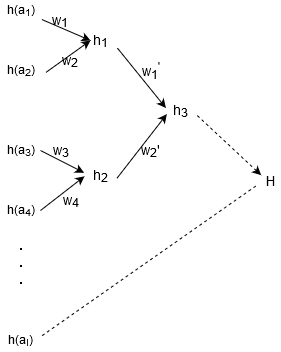
\includegraphics[scale=0.6]{Grafiken/HerdingAttack.png}
\label{pic:herdingattack}
\caption{Dieser Hashbaum gibt Pfade an um aus $2^k$ Hashes den gewünschten Hash durch Konkatenation der Strings zu erreichen.}
\end{figure}

\begin{figure}[h!]
\centering
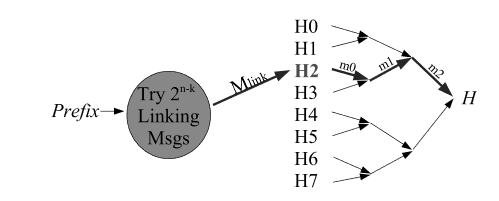
\includegraphics[scale=0.6]{Grafiken/HerdingAttack2_Linking.png}
\label{png:herdinglinking}
\caption{Nachdem ein Linkender String gefunden wurde, kann die gefälschte Nachricht zusammengesetzt werden}
\end{figure}
Ist die Menge an möglichen Präfixen im vorhinein bekannt, so kann die Menge an Starthashes entsprechend dieser Präfixe gewählt werden, wodurch der Aufwand für die Suche des Linkenden Strings gespart wird. Ist die Menge so groß dass nicht alle möglichen Hashkombinationen berechnet werden können, so könnte auch das Risiko einer Entarnung in Kauf genommen werden, wenn ein genügend ähnlicher Präfix verwendet wird. Des weiteren können auch sofern die zu verändernden Stellen innerhalb von abzugrenzenden Blöcken eines Dokumentes liegen, für jede einzelne Stelle eigene alternierende Texte mit den selben Hashes gefunden werden, sodass diese auch ohne eine Baumstruktur vertauscht werden können.
\subsubsection{HMAC-Konstruktion}
Sei $H: \mathbb{Z}_2^*\rightarrow\mathbb{Z}_2^{8n}$ eine Hashfunktion, $opad = (0x5C)^n=(01011100)^n\in \mathbb{Z}_2^{8n}$\\
und $ipad=(0x36)^n=(00110110)^n\in \mathbb{Z}_2^{8n}$, dann definieren wir $HMAC:\mathbb{Z}_2^*\times\mathbb{Z}_2^*\rightarrow\mathbb{Z}_2^*$ als
$$HMAC(x,k)=H\left( conc\left( K\oplus opad, H\left( conc\left( K\oplus ipad,x\right)\right)\right)\right)$$
Dabei ist die Wahl von $K\in\mathbb{Z}_2^{8n}$ von k abhängig:
\begin{itemize}
\item $|k|=8n\Rightarrow K=k$
\item $|k|=m<8n\Rightarrow K = k0^{8n-m}$, d.h. k wird auf Blockgröße aufgefüllt
\item $|k|>8n\Rightarrow K = H(k)$
\end{itemize}
Der Keyed-Hash Message Authentification Code (HMAC) hashed hierbei die Nachricht x, sodass auch bei der Verwendung einer Hashfunktion welche nicht kollisionsresistent ist das Verfahren nicht unsicher wird. Da der Hashwert der Nachricht direkt innerhalb einer Hashoperation berechnet wird, gilt die Grundlage für CTFP nicht, da hier die Berechnung nicht in unterteilten Blöcken funktioniert. $H(x)=H(x')\nRightarrow H(xS)=H(x'S)$\\
Damit ist die HMAC Konstruktion zwar effizient und eine Fälschung einer Nachricht schwierig, um die Authentizität einer Nachricht zu prüfen müssen aber beide Parteien den geheimen Schlüssel kennen um den Hash neu zu bilden und zu prüfen.\\
Varianten des HMAC sind:\\
\blue{HMAC-based One-time Password Algorithmus (HOTP)} verwendet einen Zähler welcher nach jeder Hashgeneration inkrementiert wird und bei der Hashgeneration den Schlüsssel erhöht. Anschließend wird der Hash in einen 6-10 stelligen numerischen Wert umgewandelt welcher auch von Menschen lesbar ist. Die selben Informationen müssen dem Authentifizierenden vorliegen, sodass falls dieser den Hash reproduzieren kann die Nachricht als gültig anerkannt wird. \\
\blue{Time-based One-time Password Algorithmus (TOTP)} verwendet anstelle eines Zählers einen Zeitstempel, funktioniert sonst aber wie HOTP. Um die Ungenauigkeiten nicht synchronisierter Uhren auszugleichen umfasst der Gültigkeitsraum eines TOTP Hashes oft rund 30 Sekunden, bevor der Hash ungültig wird. Das Verfahren kommt vor allem in der 2-Faktor Authentifizierung zum Einsatz.\\
\subsection{Digitale Signaturen}
Signaturen erlauben es die \hyperref[item:schutzziele]{Authentizität, Integrität und Nicht-Abstreitbarkeit} einer Nachricht zu testen bzw. sicherstellen.\\
Ein Angreifer kann keinen Schlüssel generieren, sodass damit für zwei verschiedene Nachrichten die selbe Signatur erzeugt wird.\\
Wir unterscheiden:
\begin{itemize}
\item \blue{Fortgeschrittene elektronische Signatur}
	\begin{itemize}
	\item Signatur ist eindeutig dem Unterzeichner zuordenbar
	\item Ermöglicht Identifizierung des Unterzeichners
	\item Wird unter Verwendung elektronischer Signaturerstellungsdaten erstellt, die der Unterzeichner mit einem hohen maß an Vertrauen unter seiner alleinigen Kontrolle verwenden kann
	\item Nachträgliche Veränderung unterzeichneter Daten muss erkannt werden
	\end{itemize}
\item \blue{Qualifizierte elektronische Signatur}
	\begin{itemize}
	\item Rechtliche Gleichstellung mit handschriftlicher Unterschrift
	\item Eine Signatur welche auf einem von einem Mitgliedsstaat ausgestellten Zertifikat beruht, ist in allen Mitgliedsstaaten gültig
	\end{itemize}	
\end{itemize}

\subsubsection{Wissen und Ziele von Angreifern}
Wie viel Wissen ein Angreifer hat unterscheiden wir mit folgenden Begriffen:
\begin{itemize}
\item \blue{Key-Only Attack}, hier besitzt der Angreifer nur den öffentlichen Schlüssel
\item \blue{Known Signature Attack}, hier sind mehrere Paare von Nachricht und Signatur bekannt
\item \blue{Chosen Message Attack}, der Angreifer kann im Vorfeld für beliebige selbstgewählte Nachrichten die Signatur bekommen
\item \blue{Adaptive Chosen Message Attack}, kann während des Angriffes für beliebig viele selbstgewählte Nachrichten zugehörige Signaturen bekommen
\end{itemize}
Die Ziele eines Angreifers mit folgenden Begriffen:
\begin{itemize}
\item \blue{Existential Forgery}, der Angreifer will ein gültiges Nachricht/Signatur-Paar ermitteln
\item \blue{Selective Forgery}, gültige Signatur zu einzelnen neuen, vor dem Angriff bekannten Nachrichten ermitteln
\item \blue{Universal Forgery}, gültige Signatur zu jedem beliebigen Dokument ermitteln
\item \blue{Total Break}, Angreifer bestimmt den geheimen Schlüssel 
\end{itemize}

Der stärkste Sicherheitsbegriff ist der des \textit{Existential forgery under a chosen message attack}

Ein Signaturschema gilt als \textbf{sicher}, wenn jeder Angreifer nach dem er n Nachrichten signiert hat mit \textbf{sehr hoher Wahrscheinlichkeit} keine Nachricht findet, sodass diese von den ursprünglich n verschieden ist aber die Signatur mit einer davon übereinstimmt

\subsubsection{Signieren mit RSA}

Mittels RSA kann signiert werden, denn die Ver-/Entschlüsselung kommutieren. Dazu wird zusätzlich noch eine Hashfunktion $h: A*\rightarrow \{0,...,n\}$ benötigt.\\
Die Signatur wird wie folgt erstellt: $s=D(h(m),(d,n))=\left( h(m)\right)^d\textrm{ mod }n$\\
Überprüfen lässt sie sich wie folgt: $h(m)=E(s,(e,n))=s^e\textrm{ mod }n$\\

\textbf{Beispiel Signaturvorgang mit RSA:}\\
Signieren:
\begin{enumerate}
\item Schlüsselgenerierung mit $(d,n)=(37313,241103)$ und $(e,n)=(65537,241103)$
\item Alice will die Nachricht $m$ mit $h(m)=164796$ signieren
\item Sie berechnet $s=h(m)^d\textrm{ mod }n=164796^{37313}\textrm{ mod }241103=129335$ 
\end{enumerate}
Verifizieren:
\begin{enumerate}
\item Bob besitzt $(e,n)$, sowie die Nachricht $m$ und ihre Signatur $s=129335$
\item Er berechnet $s^e\textrm{ mod }n=129335^{65537}\textrm{ mod }241103=164796$
\item Er berechnet den Hash der Nachricht $m$
\item Da beide Berechnungen das selbe Ergebnis haben, akzeptiert Bob die Signatur
\end{enumerate}
Eine Signaturerstellung mit RSA ist nur sicher, sofern RSA sicher ist.

\subsubsection{Digital Signature Algorithm}

\textbf{Parametergenerierung:}
\begin{enumerate}
\item Wähle gleichverteilt zufällig eine große Primzahl $q$ (160 Bit, 224 Bit, 256 Bit)
\item Wähle große Primzahl $p$ (1024 Bit, 2048 Bit, 3072 Bit), sodass $q|(p-1)$ gilt
\item Suche ein $g\in\mathbb{Z}_p^\times$ mit ord\footnote{Die Ordnung eines Elementes ist die Zahl ord$(g):=$ inf$\{n\in\mathbb{N}:g^n=e\}\in\mathbb{N}\cup\{\infty\}$}$(g)=q$,d.h. wir wählen $h\in\mathbb{Z}_p^\times$ mit $g:=h^{\frac{p-1}{q}}\textrm{ mod } p \neq 1$.\footnote{ Da $ggT(h,p)=1$ ist, gilt $g\equiv_p h^{\frac{p-1}{q}}\xRightarrow{\text{Kleiner Fermat}}g^q\equiv_p h^{p-1}\equiv_p 1\Rightarrow$ ord$(g)\leq q$.\\ Da $q$ prim ist kann die Ordnung von $g$ kein Teiler von $q$ sein, damit gilt ord$(g)=q$}
\item Die Parameter $p,q,g$ sind öffentlich
\end{enumerate}

\textbf{Schlüsselgenerierung:}
\begin{enumerate}
\item Wähle zufällig $x$ mit $1<x<q$
\item Berechne $y=g^x\textrm{ mod }p$
\end{enumerate}
Dann ist $y$ der öffentliche Schlüssel und $x$ der private Schlüssel.\\
Die Berechnung des privaten Schlüssel aus dem öffentlichen Schlüssel ist eine Instanz des diskreten Logarithmus, und somit nicht effizient lösbar.\\

\textbf{Signieren:}
\begin{enumerate}
\item Wähle $k$ mit $1<k<q$
\item Bestimme $r=(g^k\textrm{ mod }p)\textrm{ mod }q$. Falls $r=0$, beginne von vorne
\item Bestimme $s=k^{-1}\cdot (H(m)+r\cdot x)\textrm{ mod }q$. Falls $s=0$, beginne von vorne
\item Signatur ist das Tupel $(r,s)$
\end{enumerate}
\textbf{Verifikation:}
\begin{enumerate}
\item Ungültig, wenn $0<r<q$ oder $0<s<q$ nicht gilt
\item Berechne $w=s^{-1}$ mod $q$
\item Berechne $u_1=H(m)\cdot w$ mod $q$
\item Berechne $u_2=r\cdot w$ mod $q$
\item Berechne $v=(g^{u_1}\cdot y^{u_2}\textrm{ mod }p)$ mod $q$
\item Akzeptiere die Signatur, falls $v=r$
\end{enumerate}

%%Falls oben mehr Text hin kommt auskommentieren
\newpage

\textbf{Beispiel für DSA}\\
Parametergenerierung:
\begin{enumerate}
\item Wir wählen $q=59$ und $p=709$
\item Mit $h=5$ gilt $g:=5^{\frac{709-1}{59}}\textrm{ mod }709=20 \neq 1$
\item Also sind $(p,q,g)=(709,59,20)$ die öffentlichen Parameter
\end{enumerate}
Schlüsselgenerierung:
\begin{enumerate}
\item Wähle $x=23$ als privaten Schlüssel
\item Bestimme $y=g^x$ mod $p=20^{23}$ mod $709=186$ als öffentlicher Schlüssel
\end{enumerate}

Signieren:\\
Wir besitzen $p=709,q=59,g=20$ und $x=23$, der Hashwert unserer Nachricht ist $H(m)=16$
\begin{enumerate}
\item Wir wählen $k=36$
\item Wir bestimmen $r=(20^{36}\textrm{ mod }709)\textrm{ mod }59=31$
\item Mit $k^{-1}=41$ bestimmen wir $s=k^{-1}\cdot (H(m)+r\cdot x)\textrm{ mod }q=29889\textrm{ mod }59=35$
\item Die Signatur ist damit $(r,s)=(31,35)$
\end{enumerate}

Verifizieren:\\
Es sind $p=709,q=59,g=20,y=186,H(m)=16$ und der Signatur $(r,s)=(31,35)$
\begin{enumerate}
\item $r$ und $s$ sind gültig
\item Wir berechnen $w=s^{-1}$ mod $q=27$
\item Wir berechnen $u_1=H(m)\cdot w$ mod $q=16\cdot 27$ mod $59=19$
\item Wir berechnen $u_2=r\cdot w$ mod $q=31\cdot 27$ mod $59=19$
\item Wir berechnen $v=(g^{u_1}\cdot y^{u_2}\textrm{ mod }p)$ mod $q=(20^{19}\cdot 186^{11}$ mod $p)$ mod $q =31$
\item Da $v=r$ gilt, wird die Signatur akzeptiert
\end{enumerate}

\subsection{Schlüsselverteilung}
Wir unterscheiden verschiedene Schlüssel:\\
\blue{Langzeitschlüssel} haben eine lange Gültigkeit (1 Monat bis 1 Jahr) und werden häufig zur Authentifizierung verwendet.\\
\blue{Kurzzeitschlüssel} bzw. \blue{Sitzungsschlüssel} haben nur eine begrenzte Gültigkeit und minimieren somit das Risiko falls der Schlüssel kompromittiert wird.\\

Ob bei einem asymmetrischen System ein öffentlicher Schlüssel tatsächlich von einer bestimmten Person kommt, kann mithilfe von Zertifkaten welche von einem vertrauenswürdigen Dritten - Public Key Infrastructure (PKI) - ausgestellt werden, verifiziert werden.
Ein solches Zertifikat beinhaltet unter Anderem: Öffentlicher Schlüssel, Name, Gültigkeitszeitraum, Austeller,...\\
Das Zertifikat wird dann mit einer digitalen Signatur des Ausstellers versehen, sodass derjenige der die Authentizität des Schlüssels prüfen will trotzdem noch dem Schlüssel des Zertifikat-Ausstellers vertrauen muss oder eben der nächst \hyperref[pic:Chainoftrust]{höheren Instanz welche den Schlüssel des Zertifikats-Austellers signiert}.

\begin{figure}
\label{pic:Chainoftrust}
\centering
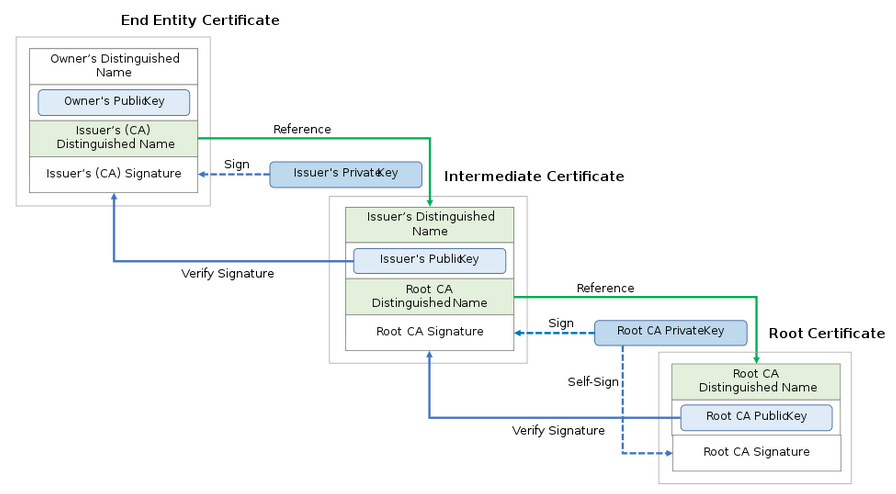
\includegraphics[scale=0.5]{Grafiken/Chain-Of-Trust.png}
\caption{Ein zentralisierter Ansatz ist X.509 als PKI, Root Certificates muss vertraut werden}
\end{figure}

Ein dezentralisierter Ansatz ist PGP, hierbei werden Schlüsselbünde versandt, sodass der Empfänger zum einen weiß welchen anderen öffentlichen Schlüsseln der Sender vertraut und dann in seinen bereits vorher empfangenen Schlüsselbändern nachsehen kann ob andere Personen denen er bereits vertraut auch dem Sender vertrauen. Falls dies der Fall ist kann er die neu erhaltenen Schlüssel als vertrauenswürdig speichern, sodass über Zeit ein Web of Trust entsteht wo alle Parteien untereinander ihre öffentlichen Schlüssel kennen. Hierbei ist aber fraglich ob Vertrauen wirklich transitiv ist.\\

Ein Problem bei beiden Ansätzen sind das ein Schlüsselverlust/-kompromittierung dafür sorgt dass die Nachrichten nicht mehr lesbar/geheim sind.\\
Als Lösung für letzteres kann ein Ablaufdatum für Zertifikate festgelegt werden oder mittels Widerrufszertifikaten vorher ausgestellte Zertifikate widerrufen werden.
Diese Widerrufszertifikate können bei X.509 von einem zentralisierten Server ausgestellt werden, wobei auch hier die Vertrauenswürdigkeit und Erreichbarkeit des Servers fragwürdig ist.
Beim Web of Trust können diese durch die Benutzer oder angegebene Parteien erstellt und verbreitet werden. Diese Updates zu verbreiten ist aber ineffizient, sollen alle alles speichern?

\subsection{Schlüsselaustausch}
Beim Man-in-the-middle Angriffsmodel hat der Angreifer vollen Zugriff auf dem Kommunikationskanal. Er kann daher:
\begin{itemize}
\item Nachrichten abfangen
\item Übermittlung von Nachrichten verzögern
\item Nachrichten unterdrücken
\item Nachrichten durch andere Nachrichten ersetzen
\item Nachrichten unter falscher Identität senden
\item Er kann aber keine kryptographische Primitive nicht brechen
\end{itemize}
\begin{figure}
\centering
\label{pic:ManInTheMiddle}
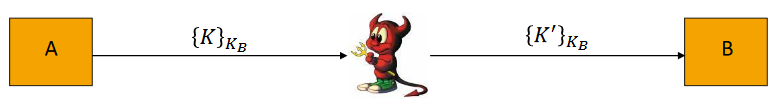
\includegraphics[scale=0.6]{Grafiken/ManInTheMiddle.png}
\caption{Man-in-the-middle Angriff, wo A einen neuen symmetrischen Schlüssel, mit öffentlichem Schlüssel $K_B$ von B verschlüsselt an B sendet, die Chiffre wird vom Angreifer abgefangen}
\end{figure}
Das \hyperref[pic:ManInTheMiddle]{naive Schlüsselaustausch Protokoll} kann um eine PKI erweitert werden, welche die öffentlichen Schlüssel von A und B kennt. A holt von T den öffentlichen Schlüssel $K_B$ von B und verschlüsselt damit den neuen Sitzungsschlüssel und schickt diesem zusammen mit seinem Namen an B. Auch hier kann ein Angreifer die Chiffre abfangen und seinen Schlüssel in Verbindung mit seinem Namen an B senden.

\subsubsection{Needham-Schroeder Protokolle}
Die \textbf{symmetrische Variante} des Protokolls läuft wie folgt ab:
\setcounter{equation}{0}
\begin{flalign}
A\rightarrow T:& A,B,N_A&&\\
T\rightarrow A:& \{ N_A,K,B,\{ K,A\}_{K_B}\}_{K_A}&&\\
A\rightarrow B:& \{ K,A\}_{K_B}&&\\
B\rightarrow A:& \{N_B\}_K&&\\
A\rightarrow B:& \{N_B-1\}_K&&
\end{flalign}
Hierbei sind $N_A$ und $N_B$ zufällig generierte Nonces. Die in Klammern geschriebene Werte werden als eine zusammengesetzte Nachricht mit dem tiefgestellten Schlüssel verschlüsselt. Dabei muss T im Besitz eines geheimen Schlüssels $K_A$ und $K_B$ zum kommunizieren mit jeweils A und B sein.\\

Indem A im ersten Schritt die gewünschten Kommunikationspartner und eine Nonce $N_A$ an den Server sendet kann dieser einen geheimen Sitzungsschlüssel $K$ generieren über den nach Abschluss des Verfahrens eine gesicherte Kommunikation zwischen A und B möglich wird. Damit die im zweiten Schritt von A empfangene Chiffre auch tatsächlich einen neuen Sitzungsschlüssel enthält muss $N_A$ neu sein, da sonst ein Angreifer eine aufgezeichnete Nachricht anstelle von T an A senden könnte um die Verwendung eines alten Schlüssels zu erzwingen. Damit außerdem kein im ersten Schritt der Empfänger nicht durch einen anderen ausgetauscht werden kann ohne das A es bemerkt sendet T auch B erneut zurück. Die innere mit $K_B$ verschlüsselte Chiffre enthält das in Schritt 3 an B gesendete Paket und kann nur von B entschlüsselt werden.\
Damit sich auch B davon überzeugen kann dass der Sitzungschlüssel $K$ neu ist sendet er eine mit K verschlüsselte Nonce $N_B$, welche A dekrementiert und zurücksendet, da $N_B$ neu ist kann auch B sicher sein, dass es sich um keinen Replay-Angriff handelt\footnote{Eine Angriffsform wo ein Angreifer zuvor aufgezeichnete Daten sendet um die Identität des vorherigen Gesprächpartners vorzutäuschen}.\\
Leider obliegt die Schlüsselgenerierung dem Knoten T auch kennt T nun den Sitzungsschlüssel.

\begin{figure}
\centering
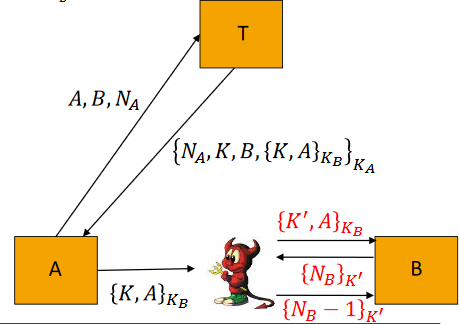
\includegraphics[scale=0.6]{Grafiken/NeedhamSchroederSymmetrisch.png}
\caption{Die symmetrische Variante des Needham-Schroeder-Schlüsselaustausches, falls der Angreifer ein altes Paar $\{K',A\}_{K_B}$ und $K'$ kennt kann der Angreifer die Indentität von A annehmen}
\end{figure}

In der \textbf{antisymmetrische Variante} funktioniert der Datenaustausch wie folgt:
\setcounter{equation}{0}
\begin{flalign}
A\rightarrow T:& A,B&&\\
T\rightarrow A:& \{K_{PB},B\}_{K_{ST}}&&\\
A\rightarrow B:& \{N_A,A\}_{K_{PB}}&&\\
B\rightarrow T:& B, A&&\\
T\rightarrow B:& \{K_{PA},A\}_{K_{ST}}&&\\
B\rightarrow A:& \{N_A,N_B\}_{K_{PA}}&&\\
A\rightarrow B:& \{N_B\}_{K_{PB}}&&
\end{flalign}

Hierbei sind $K_{PA}$ und $K_{PB}$ die öffentlichen Schlüssel von A bzw. B, sowie $K_{ST}$ der private Signaturschlüssel von T.

\subsubsection{Diffie-Hellman-Protokoll}
Zu Beginn muss eine Primzahl $p$ und ein Generator $g\in \mathbb{Z}_p^\times$ für eine Gruppe $\mathbb{Z}_p$ gemeinsam gewählt werden. Dann läuft das Verfahren wie folgt ab:
\begin{enumerate}
\item A wählt $a\in\mathbb{N}$ mit $0<a<p$ zufällig und sendet $g^a$ mod $p$ an B
\item B wählt $b\in \mathbb{N}$ mit $<b<p$ zufällig und sendet $g^b$ mod $p$ an A
\item A berechnet $(g^b)^a$ mod $p$
\item B berechnet $(g^a)^b$ mod $p$
\end{enumerate}
Damit haben A und B den selben Schlüssel $g^{ab}$ und können darüber kommunizieren. Ein passiver Angreifer, d.h. ein Angreifer welcher nur den Datenaustausch mithören kann $a$ oder $b$ nicht einfach berechnen.\\
Allerdings wurde früher oft nur eine geringe Menge an Primzahlen für p verwendet, sodass die möglichen Logarithmen vorberechnet werden konnten. Zwei Vorberechnungen deckten $66$\% der IPsec-VPNs und $26$\% der SSH-Server ab.
Bei einem MitM-Angriff kann der Angreifer damit parallel zwei DH-Protokolle laufen lassen und so Schlüssel selber wählen.
Als Lösung hierfür können die Nachrichten signiert werden \blue{authenticated DH/Station-to-Station-Protokoll}.\\

Für das Station-to-Station-Protokoll (STS) müssen beide Parteien einen Signaturschlüssel $sk_A$ und $sk_B$ besitzen und die Zertifikate der Schlüssel sind beiden bekannt. Wir bezeichnen $K=g^{ab}$
\setcounter{equation}{0}
\begin{flalign}
A\rightarrow B: & g^a&&\\
B\rightarrow A: &g^b,\{sig(sk_B,(g^a,g^b))\}_K&&\\
A\rightarrow B: & \{sig(sk_A,(g^a,g^b))\}_K &&
\end{flalign}
\end{document}